%\documentclass[11pt,a4paper]{article}
\documentclass[11pt
  , a4paper
  , article
  , oneside
%  , twoside
%  , draft
]{memoir}

\usepackage{control}
\usepackage[numbers]{natbib}

\begin{document}

\newcommand{\technumber}{
  RAON Control-Document Series\\
  Revision : v1.0,   Release : a fixed date}
\title{\textbf{Raspberry Pi Technical Documentation}}

\author{scwook\thanks{@ibs.re.kr} \\

  Rare Isotope Science Project\\
  Institute for Basic Science, Daejeon, South Korea
}
\date{\today}

\renewcommand{\maketitlehooka}{\begin{flushright}\textsf{\technumber}\end{flushright}}
%\renewcommand{\maketitlehookb}{\centering\textsf{\subtitle}}
%\renewcommand{\maketitlehookc}{C}
%\renewcommand{\maketitlehookd}{D}

\maketitle

\begin{abstract}
본 기술문서는 Raspberry Pi에 대한 기본 설치 및 설정방법을 포함하여 다양한 센서들을 이용한 테스트 및 
EPICS Integration 방법에 대하여 설명하였다. 기본적으로 사용된 Model은 Raspberry Pi Model B+ 이며  
OS는 Raspbian을 사용하였다. \citep{FAI}
\end{abstract}

\chapter{Introduction}
Raspberry Pi(RPi)는 교육용 프로젝트의 일환으로 개발된 소형 컴퓨터로 가격이 아주 저렴하고 신용카드 정도의
크기를 가지고 있다. RPi는 하드웨어적으로 ARM기반의 CPU를 장착하고 있으며 5V의 Micro USB를 통해 전원을 
공급받는다. 확장 포트로는 USB, Ethernet Port, HDMI를 지원하며, 특히 입출력 신호를 제어하기 위한 
GPIO(General Purpose Inut Output)포트를 지원하는데 SPI, I2C, UART통신이 가능하다. 결과적으로 다양한
Device 및 Sensor를 RPi를 통해 제어 및 모니터링 가능하다.\\

RPi는 ARM 아키텍쳐를 기반으로 하기 때문에 이를 지원하는 OS는 거의 설치가능하다. 현재 공식 홈페이지에서
제공하는 OS는 5가지가 있으며, 이 중 Debian 계열의 Raspbian이 가장 많이 사용되고 있다.

\section{Installation}
Raspbian을 설치하는 방법은 2가지가 있다.
\begin{itemize}
\item New Out Of the Box Software(NOOBS) 설치
\item Raspbian Image 설치
\end{itemize}
Raspberry Pi에 설치되는 OS는 Raspbian외에 몇가지가 더 있는데 NOOBS는 이러한 OS를 Package로 묶은 것으로 
하나 또는 그 이상의 OS를 한번에 설치할 수 있다. 만약 하나의 OS만 설치하고자 하는 경우에는 Image파일을 
이용하여 설치하면 되는데 초보자에게는 다소 어려울 수 있다. RPi 공식 홈페이지에서는 NOOBS를 이용하는 것을 추천함으로 여기에서도 NOOBS를 이용하여 설치를 진행한다.
\subsection{Download}
Raspbian 설치를 위해 다음 홈페이지에서 NOOBS 파일을 다운 받는다\\
http://www.raspberrypi.org/downloads/\\
다운로드한 파일의 압축을 해제하고 Micro SD Card에 파일을 전부 복사한다.\\
\subsection{First Boot}
Raspberry Pi전원을 연결 하면 그림\ref{fig:noobs_manager}와 같은 NOOBS Install Manager가 나오는데 
Raspbian을 선택한 후 Install 버튼을 
누르면 설치가 진행된다. 설치가 완료되고 재부팅을 하면 그림\ref{fig:raspi_conf}와 같이 
Raspberry Pi Software Configuration Tool이 나타나고 Finish를 누르면 기본적인 Raspbian 설치는 완료된다.
\begin{figure}[!htb]
\centering
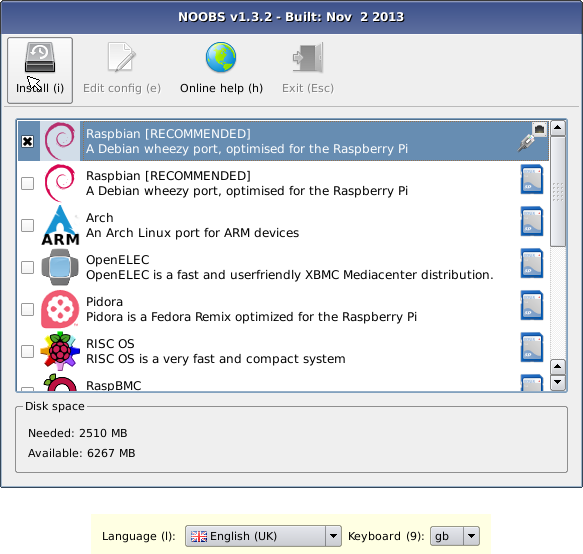
\includegraphics[width=1\textwidth]{./images/raspberry/noobs.png}
\caption{NOOBS Install Manager}
\label{fig:noobs_manager}
\end{figure}

\begin{figure}[!htb]
\centering
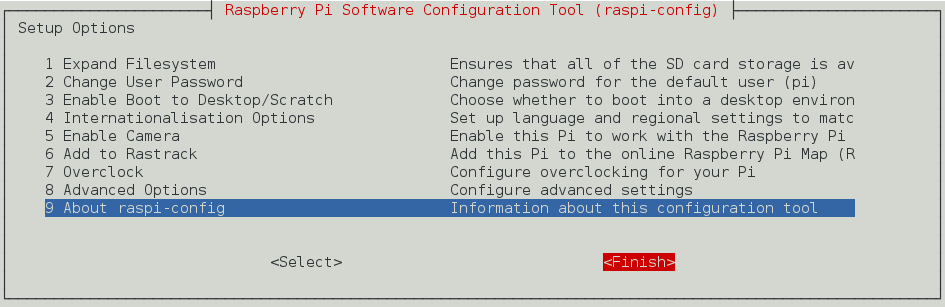
\includegraphics[width=1\textwidth]{./images/raspberry/rasp_config.png}
\caption{Raspberry Pi Software Configuration Tool}
\label{fig:raspi_conf}
\end{figure}

\section{Configuration}
\subsection{Password 변경}
Raspbian의 기본 ID 및 Password는 각각 pi와 raspberry로 설정되어 있다. 기본 Password 는 passwd
명령을 통해 변경 가능하다.
\begin{lstlisting}[style=termstyle]
pi@raspberry# passwd
Changing password for pi.
(current) UNIX password: 
Enter new UNIX password: 
Retype new UNIX password: 
passwd: password updated successfully
\end{lstlisting}

\subsection{Networking}
네트워크는 기본적으로 DHCP로 설정되어 있다. 고정 IP로 변경할 경우 /etc/network/interface 파일을 수정한다.
\begin{lstlisting}[style=termstyle]
auto lo

iface lo inet loopback

allow-hotplug eth0
iface eth0 inet static
        address 10.1.4.206
        netmask 255.255.255.0
        broadcast 10.1.4.255
        gateway 10.1.4.254
        dns-nameservers 10.1.2.240
\end{lstlisting}
무선 네트워크를 사용할 경우 다음과 같이 무선 네트워크 정보를 추가해 준다.
\begin{lstlisting}[style=termstyle]
auto lo

iface lo inet loopback

allow-hotplug wlan0
iface wlan0 inet static
	address 10.1.4.207
	netmask 255.255.255.0
	network 10.1.4.0
	broadcast 10.1.4.255
	gateway 10.1.4.254
	dns-nameservers 10.1.2.240
	wpa-scan-ssid 1
	wpa-ap-ssid 1
	wpa-key-mgmt WPA-PSK
	wpa-proto RSN WPA
	wpa-pairwise CCMP TKIP
	wpa-group CCMP TKIP
	wpa-ssid "CTRLTEAM"
	wpa-psk "rkthrrlwpdj"
\end{lstlisting}
여기서 wpa-ssid와 wpa-psk는 사용하고자 하는 무선네트워크 ssid와 password를 넣으면 된다. 만약 DHCP로
무선을 설정 할 경우 다음과 같이 wpa-ssid와 wpa-psk만 설정해 주면 된다.
\begin{lstlisting}[style=termstyle]
auto lo

iface lo inet loopback

allow-hotplug wlan0
iface wlan0 inet dhcp
        wpa-ssid "CTRLTEAM"
        wpa-psk "rkthrrlwpdj"
\end{lstlisting}

\section{Library}
\subsection{wiringPi}
WiringPi는 Arduino에서 사용되는 Wiring Library를 RPi에 맞게 변경한 것으로 GPIO access를 포함하여 
PiFace, GertBoard와 같은 확장 보드 및 HD44780U와 같은 Device Chip을 지원한다. 보다 자세한 사항은
홈페이지를 참고하기 바란다.\\

Wiring Pi 설치는 git 서버로 부터 파일을 복사한 후 빌드하면 된다.
\begin{lstlisting}[style=termstyle]
pi@raspberry# git clone git://git.drogon.net/wiringPi
Cloning into 'wiringPi'...
remote: Counting objects: 657, done.
remote: Compressing objects: 100% (599/599), done.
remote: Total 657 (delta 476), reused 95 (delta 58)
Receiving objects: 100% (657/657), 247.61 KiB | 94 KiB/s, done.
Resolving deltas: 100% (476/476), done.
pi@raspberrypi# cd wiringPi
pi@raspberrypi:/wiringPi# ./build
\end{lstlisting}
Pin Layout은 'readall' 명령으로 확인 가능하다. Wiring Pi는 자체적인 Pin Map을 사용하는데 wPi로 
표시된 부분은 Wiring Pi에서 사용하는 GPIO 핀 번호이다.
\begin{lstlisting}[style=termstyle]
pi@raspberrypi# gpio readall
+-----+-----+---------+------+---+--B Plus--+---+------+---------+-----+-----+
 | BCM | wPi |   Name  | Mode | V | Physical | V | Mode | Name    | wPi | BCM |
 +-----+-----+---------+------+---+----++----+---+------+---------+-----+-----+
 |     |     |    3.3v |      |   |  1 || 2  |   |      | 5v      |     |     |
 |   2 |   8 |   SDA.1 |   IN | 1 |  3 || 4  |   |      | 5V      |     |     |
 |   3 |   9 |   SCL.1 |   IN | 1 |  5 || 6  |   |      | 0v      |     |     |
 |   4 |   7 | GPIO. 7 |   IN | 0 |  7 || 8  | 1 | ALT0 | TxD     | 15  | 14  |
 |     |     |      0v |      |   |  9 || 10 | 1 | ALT0 | RxD     | 16  | 15  |
 |  17 |   0 | GPIO. 0 |   IN | 0 | 11 || 12 | 0 | IN   | GPIO. 1 | 1   | 18  |
 |  27 |   2 | GPIO. 2 |   IN | 0 | 13 || 14 |   |      | 0v      |     |     |
 |  22 |   3 | GPIO. 3 |   IN | 0 | 15 || 16 | 0 | IN   | GPIO. 4 | 4   | 23  |
 |     |     |    3.3v |      |   | 17 || 18 | 0 | IN   | GPIO. 5 | 5   | 24  |
 |  10 |  12 |    MOSI |   IN | 0 | 19 || 20 |   |      | 0v      |     |     |
 |   9 |  13 |    MISO |   IN | 0 | 21 || 22 | 0 | IN   | GPIO. 6 | 6   | 25  |
 |  11 |  14 |    SCLK |   IN | 0 | 23 || 24 | 0 | IN   | CE0     | 10  | 8   |
 |     |     |      0v |      |   | 25 || 26 | 0 | IN   | CE1     | 11  | 7   |
 |   0 |  30 |   SDA.0 |   IN | 0 | 27 || 28 | 0 | IN   | SCL.0   | 31  | 1   |
 |   5 |  21 | GPIO.21 |   IN | 0 | 29 || 30 |   |      | 0v      |     |     |
 |   6 |  22 | GPIO.22 |   IN | 0 | 31 || 32 | 0 | IN   | GPIO.26 | 26  | 12  |
 |  13 |  23 | GPIO.23 |   IN | 0 | 33 || 34 |   |      | 0v      |     |     |
 |  19 |  24 | GPIO.24 |   IN | 0 | 35 || 36 | 0 | IN   | GPIO.27 | 27  | 16  |
 |  26 |  25 | GPIO.25 |   IN | 0 | 37 || 38 | 0 | IN   | GPIO.28 | 28  | 20  |
 |     |     |      0v |      |   | 39 || 40 | 0 | IN   | GPIO.29 | 29  | 21  |
 +-----+-----+---------+------+---+----++----+---+------+---------+-----+-----+
 | BCM | wPi |   Name  | Mode | V | Physical | V | Mode | Name    | wPi | BCM |
 +-----+-----+---------+------+---+--B Plus--+---+------+---------+-----+-----+
\end{lstlisting}

\begin{figure}
  \centering
  \subbottom[Model B]
  {
    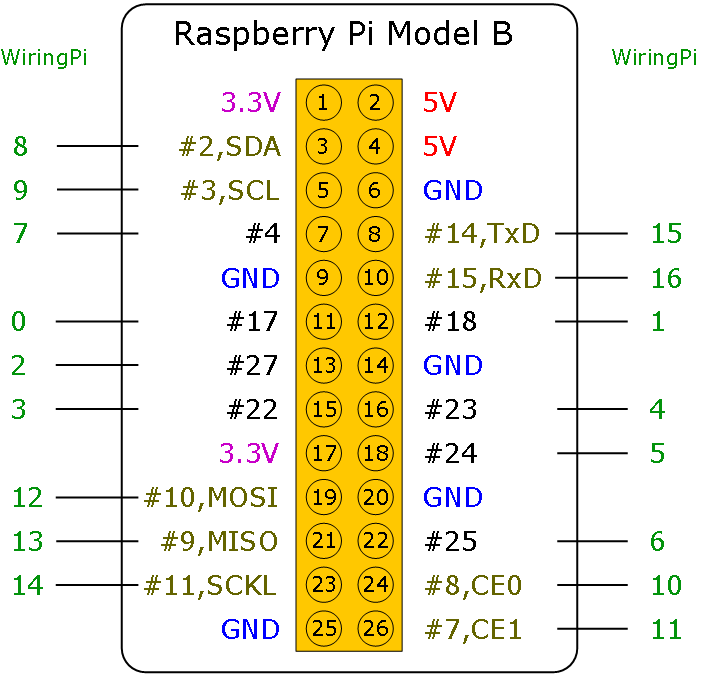
\includegraphics[width=175px]{./images/raspberry/pinmapb.png}
    \label{fig:pin_b}
  }
  \hfill
  \subbottom[Model B+]
  {
    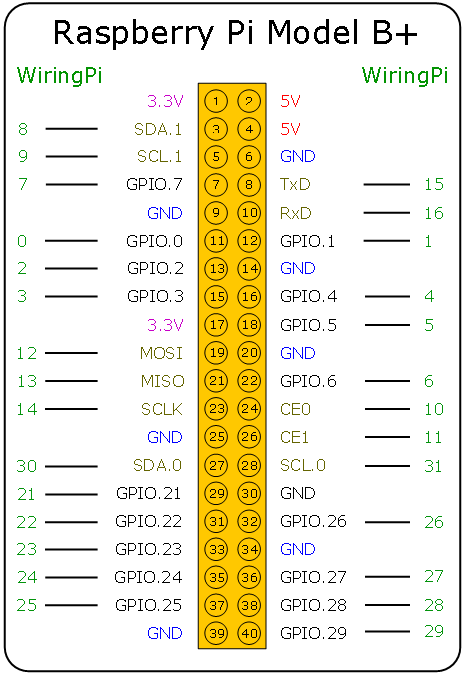
\includegraphics[width=116px]{./images/raspberry/pinmapbp.png}
    \label{fig:pin_bp}
  }
  \caption{Raspberry Pi Pin Map}
  \label{fig:rpi_pin_map}
\end{figure}

\chapter{Application}
본 Chapter에서는 RPi에 연결 가능한 Device 및 Sensor를 이용한 테스트 설명한다. 테스트는 Model B+에서
진행되었으며 기본적으로 Rasbian 과 wiringPi가 설치되어 있어야한다.

\subsection{DS1820}
DS1820 센서를 이용하여 온도를 읽어 보자.
\begin{figure}[!htb]
\centering
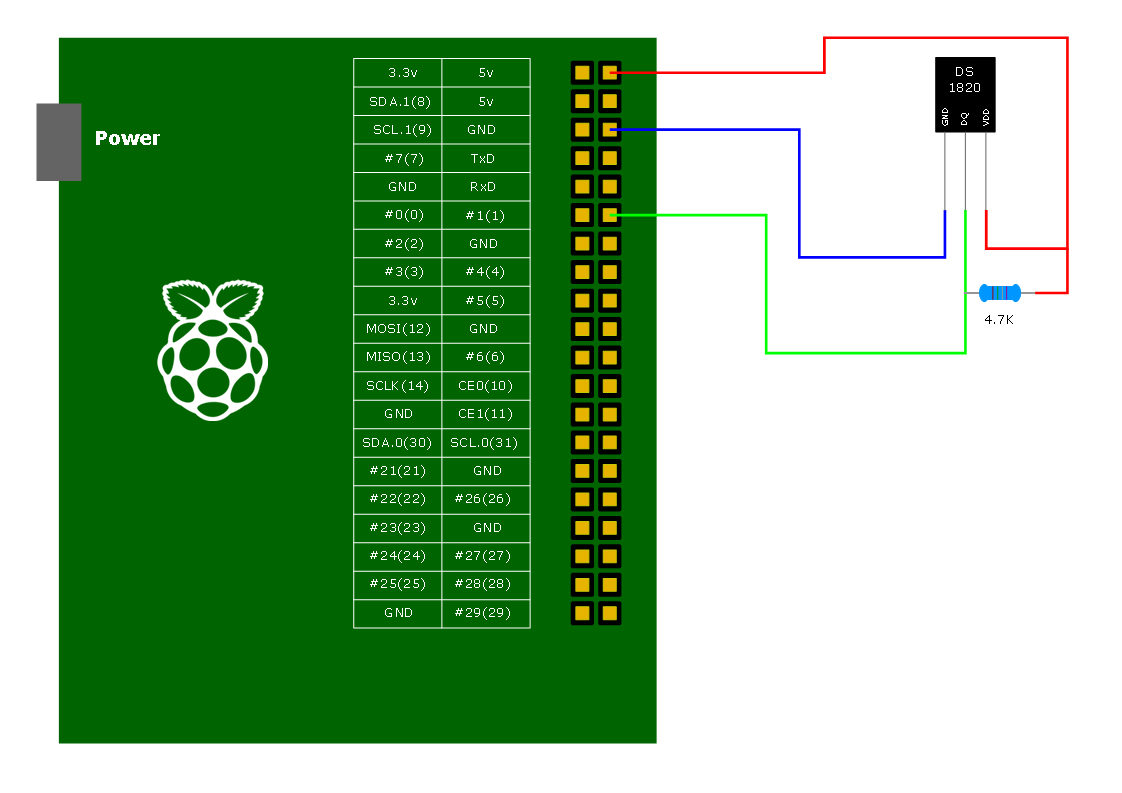
\includegraphics[width=1\textwidth]{./images/raspberry/ds1820_test.png}
\caption{DS1820 Temperature Sensor Test}
\label{fig:ds1820_test}
\end{figure}
소스코드는 다음과 같다.
\begin{lstlisting}[style=termstylenumber, caption={Editing \texttt{/etc/fai/NFSROOT}}, label={list:nfsroot-file}]
#include <stdio.h>
#include <string.h>
#include <stdlib.h>
#include <stdint.h>

#include <wiringPi.h>

#define PIN_NUM 1

float ds1820_read();
int onewire_reset();
void onewire_write(uint8_t data);
void onewire_write_bit(int bit);
uint8_t onewire_read();
int onewire_read_bit();
uint8_t crc_read();
uint8_t crc_cal(uint8_t crc, uint8_t data);

int main()
{
  if(wiringPiSetup() == -1)
    return 1;

  float temp = 0.0f;

  while(1)
  {
    temp = ds1820_read();
    printf("%.1f\n", temp);

   delay(1000);
  }
}
float ds1820_read()
{
  uint8_t busy = 1;

  onewire_reset();
  onewire_write(0xCC);
  onewire_write(0x44);

  delay(750);
  while(busy == 0)
  {
    busy = onewire_read();
    printf("busy: %d\n", busy);
  }

  onewire_reset();
  onewire_write(0xCC);
  onewire_write(0xBE);

  uint8_t lsb, msb, th, tl, reserved1, reserved2, count_remain, count_per_c, crc;
  float real_temp = 0.0f;
  signed char temp_read = 0;

  lsb = onewire_read();
  msb = onewire_read();
  th = onewire_read();
  tl = onewire_read();
  reserved1 = onewire_read();
  reserved2 = onewire_read();
  count_remain = onewire_read();
  count_per_c = onewire_read();
  crc = onewire_read();

  uint8_t data[] = {lsb, msb, th, tl, reserved1, reserved2, count_remain, count_per_c};

  onewire_reset();

  if(crc_read(data) == crc)
  {
    temp_read = (signed char)(lsb>>1);

    if(msb == 255)
      temp_read = temp_read | 0x80;

    real_temp = (float)temp_read + 0.85f - (float)count_remain/(float)count_per_c;
    real_temp = (int)(real_temp * 10) / 10.0f;
  }
  else
    printf("CRC Error  ");

  return real_temp;
}

int onewire_reset()
{
  int result;

  pinMode(PIN_NUM, OUTPUT);

  digitalWrite(PIN_NUM, LOW);
  delayMicroseconds(480);

  pinMode(PIN_NUM, INPUT);
  delayMicroseconds(70);

  result = digitalRead(PIN_NUM);

  delayMicroseconds(410);

  return result;
}

void onewire_write(uint8_t data)
{
  int loop;

  for(loop=0; loop<8; loop++)
  {
    onewire_write_bit(data & 0x01);

    data >>= 1;
  }
}
void onewire_write_bit(int bit)
{
  pinMode(PIN_NUM, OUTPUT);

  if(bit)
  {
    digitalWrite(PIN_NUM, LOW);
    delayMicroseconds(6);
    digitalWrite(PIN_NUM, HIGH);
    delayMicroseconds(64);
  }
  else
  {
    digitalWrite(PIN_NUM, LOW);
    delayMicroseconds(60);
    digitalWrite(PIN_NUM, HIGH);
    delayMicroseconds(10);
  }

}

uint8_t onewire_read()
{
  int loop, result=0;

  for(loop=0; loop<8; loop++)
  {
    result >>= 1;

    if(onewire_read_bit())
      result |= 0x80;
  }

  return result;
}

int onewire_read_bit()
{
  int result;

  pinMode(PIN_NUM, OUTPUT);

  digitalWrite(PIN_NUM, LOW);
  delayMicroseconds(6);

  pinMode(PIN_NUM, INPUT);
  delayMicroseconds(9);

  result = digitalRead(PIN_NUM) & 0x01;
  delayMicroseconds(55);

  return result;
}

uint8_t crc_read(uint8_t *data)
{
 uint8_t i, crc;

 crc = 0x00;

 for(i=0; i<8; i++)
  crc = crc_cal(crc, data[i]);

 return crc;
}

uint8_t crc_cal(uint8_t crc, uint8_t data)
{
  int j;
  for(j=0;j<8;j++) {
      if ((data & 0x01 ) ^ (crc & 0x01)) {
	  // DATA ^ LSB CRC = 1
	  crc = crc>>1;
	  // Set the MSB to 1
	  crc = crc | 0x80;
	  // Check bit 3
	  if (crc & 0x04) {
	      crc = crc & 0xFB; // Bit 3 is set, so clear it
	  } else {
	      crc = crc | 0x04; // Bit 3 is clear, so set it
	  }
	  // Check bit 4
	  if (crc & 0x08) {
	      crc = crc & 0xF7; // Bit 4 is set, so clear it
	  } else {
	      crc = crc | 0x08; // Bit 4 is clear, so set it
	  }
      } else {
	  // DATA ^ LSB CRC = 0
	  crc = crc>>1;
	  // clear MSB
	  crc = crc & 0x7F;
	  // No need to check bits, with DATA ^ LSB CRC = 0, they will remain unchanged
      }
      data = data>>1;
  }

  return crc;
}
\end{lstlisting}
컴파일 후 실행한다.
\begin{lstlisting}[style=termstyle]
pi@raspberrypi# gcc -o ds1820 ds1820.c -lwiringPi
pi@raspberrypi# sudo ./ds1820
\end{lstlisting}
온도 값이 출력되면 성공
\chapter{EPICS Integration}
\section{GPIO}
Raspberry Pi는 40개의 입출력 Pin을 가지고 있는데(Model B의 경우 26개) 여기에서는 GPIO를 EPICS 에서 
사용하기 위한 방법과 테스트 과정에 대하여 설명하였다.\\
EPICS Application 폴더를 생성한다. 
\begin{lstlisting}[style=termstyle]
pi@ctrlpi3 cd ../epics/R3.14.12.4/siteApps
pi@ctrlpi3 ~/epics/R3.14.12.4/siteApps# mkdir gpio
pi@ctrlpi3 ~/epics/R3.14.12.4/siteApps# cd gpio
pi@ctrlpi3 ~/epics/R3.14.12.4/siteApps/gpio# makeBaseApp.pl -t ioc gpio
pi@ctrlpi3 ~/epics/R3.14.12.4/siteApps/gpio# makeBaseApp.pl -i -t ioc gpio

Using target architecture linux-arm (only one available)
The following applications are available:
    gpio
What application should the IOC(s) boot?
The default uses the IOC's name, even if not listed above.
Application name? gpio
pi@ctrlpi3 ~/epics/R3.14.12.4/siteApps/gpio# ls
conigure  gpioApp  iocBoot Makefile
\end{lstlisting}
gpioApp/src 폴더로 이동한 후 devGPIO.c 파일을 만들어 기본 코드를 작성한다.
\begin{lstlisting}[style=termstylenumber, caption={Editing \texttt{/etc/fai/NFSROOT}}, label={list:nfsroot-file}]
#include <stdio.h>
#include <string.h>
#include <stdlib.h>

#include <epicsExport.h>
#include <devSup.h>
#include <boRecord.h>
#include <biRecord.h>

#include <wiringPi.h>

static long bo_init_record(boRecord *pbo);
static long bi_init_record(biRecord *pbi);

static long write_bo(boRecord *pbo);
static long read_bi(biRecord *pbi);

static long bo_init_record(boRecord *pbo)
{
}

static long bi_init_record(biRecord *pbi)
{
}

static long write_bo(boRecord *pbo)
{
}

static long read_bi(biRecord *pbi)
{
}

struct
{
  long num;
  DEVSUPFUN     report;
  DEVSUPFUN     init;
  DEVSUPFUN     init_record;
  DEVSUPFUN     get_ioint_info;
  DEVSUPFUN     write_bo;
  DEVSUPFUN     special_linconv;
} devBoGpioAsync = {
  6,
  NULL,
  NULL,
  bo_init_record,
  NULL,
  write_bo,
  NULL
};

struct
{
  long num;
  DEVSUPFUN     report;
  DEVSUPFUN     init;
  DEVSUPFUN     init_record;
  DEVSUPFUN     get_ioint_info;
  DEVSUPFUN     read_bi;
  DEVSUPFUN     special_linconv;
} devBiGpioAsync = {
  6,
  NULL,
  NULL,
  bi_init_record,
  NULL,
  read_bi,
  NULL
};

epicsExportAddress(dset,devBoGpioAsync);
epicsExportAddress(dset,devBiGpioAsync);
\end{lstlisting}

\section{Humidity and Temperature Sensor}
Record는 출력을, biRecord는 입력을 위한 Record이며, 각각의 Record에 대한 초기화 함수와 GPIO를 
읽고 쓰기 위한 함수로 구성되어 있다. dset을 devBoGpioAsync와 devBiGpioAsync로 설정 하였으므로 
devGPIO.dbd 파일을 만들어 다음과 같이 작성한다. 
\begin{lstlisting}[style=termstyle]
device(bo, INST_IO, devBoGpioAsync, "GPIO")
device(bi, INST_IO, devBiGpioAsync, "GPIO")
\end{lstlisting}
기본 구조가 완성되었으면 실제 코드를 작성하도록 한다. 우선 초기화 함수를 다음과 같이 작성한다.
\begin{lstlisting}[style=termstylenumber, caption={Editing \texttt{/etc/fai/NFSROOT}}, label={list:nfsroot-file}]
static long bo_init_record(boRecord *pbo)
{
  struct Pin_Info *pin_info = malloc(sizeof(struct Pin_Info));

  if(wiringPiSetup() == -1)
    return 1;

  int pin_num = 0;
  pin_num = atoi(pbo->out.value.instio.string);

  pinMode(pin_num, OUTPUT);

  pin_info->pin_num = pin_num;

  pbo->dpvt = pin_info;

  return 0;
}

static long bi_init_record(biRecord *pbi)
{
  struct Pin_Info *pin_info = malloc(sizeof(struct Pin_Info));

  if(wiringPiSetup() == -1)
    return 1;

  int pin_num = 0;
  pin_num = atoi(pbi->inp.value.instio.string);

  pinMode(pin_num, INPUT);

  pin_info->pin_num = pin_num;

  pbi->dpvt = pin_info;

  return 0;
}
\end{lstlisting}
핀 번호를 저장하기 위한 구조체를 함수 선언 아래에 해준다.
\begin{lstlisting}[style=termstylenumber, caption={Editing \texttt{/etc/fai/NFSROOT}}, label={list:nfsroot-file}]
...
...
static long write_bo(boRecord *pbo);
static long read_bi(biRecord *pbi);

struct Pin_Info
{
  int pin_num;
}; 
\end{lstlisting}
bo와 bi초기화 코드는 거의 동일하며 차이는 bo의 경우 Link를 out에서, bi의 경우 Link를 inp에서 가져온다. 
또한 bo는 출력이므로 pinMode를 OUTPUT으로 설정하며 bi는 입력 모드인 INPUT로 설정한다.\\
초기화 함수가 완료되었으면 실제 값을 읽고 쓰는 함수를 작성한다. 우선 write\_bo 함수를 작성한다.
\begin{lstlisting}[style=termstylenumber, caption={Editing \texttt{/etc/fai/NFSROOT}}, label={list:nfsroot-file}]
static long write_bo(boRecord *pbo)
{
  struct Pin_Info *pin_info = pbo->dpvt;

  int pin = pin_info->pin_num;
  int val = pbo->rval;

  digitalWrite(pin, val);

  return 0;
}
\end{lstlisting}
GPIO 출력을 위해 wiringPi Library에 있는 digitalWrite 함수를 사용하는데 이 함수는 출력하고자 
하는 핀 번호와 출력값을 함수 인자로 받는다. 핀 번호는 앞서 dpvt 포인터에 저장된 구조체를 이용하여 
읽어온다. 출력 값은 boRecord 구조체 안에있는 rval변수로 부터 알 수 있다. 즉, 사용자가 다음과 같이 
값을 설정하면 그 값이 rval에 저장된다. 
\begin{lstlisting}[style=termstyle]
scwook@scwook:# caput out4 1
\end{lstlisting}
다음은 read\_bi 함수를 작성한다.
\begin{lstlisting}[style=termstylenumber, caption={Editing \texttt{/etc/fai/NFSROOT}}, label={list:nfsroot-file}]
static long read_bi(biRecord *pbi)
{
  struct Pin_Info *pin_info = pbi->dpvt;

  int pin = pin_info->pin_num;
  int val = digitalRead(pin);

  pbi->rval = val;

  return 0;
}
\end{lstlisting}
read\_bi함수는 write\_bo함수와 구조는 같으며 핀 값을 읽어들이는 digitalRead함수를 사용한다. 
이 함수는 핀 번호를 함수 인자로 받아 현재 핀 상태가 HIGH면 1, LOW면 0값을 리턴한다.\\
전체 코드는 다음과 같다.
\begin{lstlisting}[style=termstylenumber, caption={Editing \texttt{/etc/fai/NFSROOT}}, label={list:nfsroot-file}]
#include <stdio.h>
#include <string.h>
#include <stdlib.h>

#include <epicsExport.h>
#include <devSup.h>
#include <boRecord.h>
#include <biRecord.h>

#include <wiringPi.h>

static long bo_init_record(boRecord *pbo);
static long bi_init_record(biRecord *pbi);

static long write_bo(boRecord *pbo);
static long read_bi(biRecord *pbi);

struct Pin_Info
{
  int pin_num;
};

static long bo_init_record(boRecord *pbo)
{
  struct Pin_Info *pin_info = malloc(sizeof(struct Pin_Info));

  if(wiringPiSetup() == -1)
    return 1;

  int pin_num = 0;
  pin_num = atoi(pbo->out.value.instio.string);

  pinMode(pin_num, OUTPUT);

  pin_info->pin_num = pin_num;

  pbo->dpvt = pin_info;

  return 0;
}

static long bi_init_record(biRecord *pbi)
{
  struct Pin_Info *pin_info = malloc(sizeof(struct Pin_Info));

  if(wiringPiSetup() == -1)
    return 1;

  int pin_num = 0;
  pin_num = atoi(pbi->inp.value.instio.string);

  pinMode(pin_num, INPUT);

  pin_info->pin_num = pin_num;

  pbi->dpvt = pin_info;

  return 0;
}


static long write_bo(boRecord *pbo)
{
  struct Pin_Info *pin_info = pbo->dpvt;

  int pin = pin_info->pin_num;
  int val = pbo->rval;

  digitalWrite(pin, val);

  return 0;
}

static long read_bi(biRecord *pbi)
{
  struct Pin_Info *pin_info = pbi->dpvt;

  int pin = pin_info->pin_num;
  int val = digitalRead(pin);

  pbi->rval = val;

  return 0;
}

struct
{
  long num;
  DEVSUPFUN     report;
  DEVSUPFUN     init;
  DEVSUPFUN     init_record;
  DEVSUPFUN     get_ioint_info;
  DEVSUPFUN     write_bo;
  DEVSUPFUN     special_linconv;
} devBoGpioAsync = {
  6,
  NULL,
  NULL,
  bo_init_record,
  NULL,
  write_bo,
  NULL
};

struct
{
  long num;
  DEVSUPFUN     report;
  DEVSUPFUN     init;
  DEVSUPFUN     init_record;
  DEVSUPFUN     get_ioint_info;
  DEVSUPFUN     read_bi;
  DEVSUPFUN     special_linconv;
} devBiGpioAsync = {
  6,
  NULL,
  NULL,
  bi_init_record,
  NULL,
  read_bi,
  NULL
};

epicsExportAddress(dset,devBoGpioAsync);
epicsExportAddress(dset,devBiGpioAsync);
\end{lstlisting}
코드 작성이 완료되면 Makefile에 다음과 같이 추가한다.
\begin{lstlisting}[style=termstyle]
TOP=../..

include $(TOP)/configure/CONFIG

USR_INCLUDES += -I/home/pi/wiringPi/wiringPi
wiringPi_DIR += /home/pi/wiringPi/wiringPi /home/pi/wiringPi/devLib

#----------------------------------------
#  ADD MACRO DEFINITIONS AFTER THIS LINE
#=============================

#=============================
# Build the IOC application

PROD_IOC = gpio
# gpio.dbd will be created and installed
DBD += gpio.dbd

# gpio.dbd will be made up from these files:
gpio_DBD += base.dbd

# Include dbd files from all support applications:
#gpio_DBD += xxx.dbd
gpio_DBD += devGPIO.dbd

# Add all the support libraries needed by this IOC
#gpio_LIBS += xxx
gpio_LIBS += wiringPi

# gpio_registerRecordDeviceDriver.cpp derives from gpio.dbd
gpio_SRCS += gpio_registerRecordDeviceDriver.cpp
gpio_SRCS += devGPIO.c

# Build the main IOC entry point on workstation OSs.
gpio_SRCS_DEFAULT += gpioMain.cpp
gpio_SRCS_vxWorks += -nil-

# Add support from base/src/vxWorks if needed
#gpio_OBJS_vxWorks += $(EPICS_BASE_BIN)/vxComLibrary

# Finally link to the EPICS Base libraries
gpio_LIBS += $(EPICS_BASE_IOC_LIBS)

#===========================

include $(TOP)/configure/RULES
#----------------------------------------
#  ADD RULES AFTER THIS LINE
\end{lstlisting}
 이제 코드작성은 완료되었으므로 테스트를 위한 db파일을 만든다. gpioApp/Db 폴더로 이동한 후 gpio.db 
파일을 만든다. 
\begin{lstlisting}[style=termstyle]
record(bi, "inp1")
{
  field(DTYP, "GPIO")
  field(SCAN, "1 second")
  field(INP, "@1")
}

record(bo, "out4")
{
  field(DTYP, "GPIO")
  field(OUT, "@4")
}
\end{lstlisting}
gpio.db에서는 GPIO 1번을 입력으로 4번을 출력으로 설정했음을 알 수있다. Makefile에 db파일을 추가해 준다.
이제 컴파일을 하기 위해 gpio폴더로 이동한 후 make를 실행한다.
\begin{lstlisting}[style=termstyle]
pi@ctrlpi3 ~/epics/R3.14.12.4/siteApps/gpio# make
\end{lstlisting}
make가 완료되면 bin/linux-arm 폴더에 gpio 파일과 db 폴더에 gpio.db 파일이 만들어 진다.
이제 ioc를 실행시키기 위해 iocBoot/iocgpio 폴더로 이동 후 st.cmd파일에 gpio.db를 추가해 준다.
\begin{lstlisting}[style=termstyle]
#!../../bin/linux-arm/gpio

## You may have to change gpio to something else
## everywhere it appears in this file

< envPaths

cd ${TOP}

## Register all support components
dbLoadDatabase "dbd/gpio.dbd"
gpio_registerRecordDeviceDriver pdbbase

## Load record instances
#dbLoadTemplate "db/userHost.substitutions"
#dbLoadRecords "db/dbSubExample.db", "user=piHost"
dbLoadRecords "db/gpio.db"

## Set this to see messages from mySub
#var mySubDebug 1

## Run this to trace the stages of iocInit
#traceIocInit

cd ${TOP}/iocBoot/${IOC}
iocInit

## Start any sequence programs
#seq sncExample, "user=piHost"
\end{lstlisting}
마지막으로 st.cmd파일을 실행파일로 변경한 후 실행시킨다.
\begin{lstlisting}[style=termstyle]
pi@ctrlpi3 ~/epics/R3.14.12.4/siteApps/gpio/iocBoot/iocdht11 $ chmod 755 st.cmd
pi@ctrlpi3 ~/epics/R3.14.12.4/siteApps/gpio/iocBoot/iocdht11 $ sudo ./st.cmd
\end{lstlisting}
out4 출력값을 1로 했을 때 LED에 불이오면 성공!
\begin{lstlisting}[style=termstyle]
epics> dbpf out4 1
\end{lstlisting}
버튼을 누른 상태에서 inp1 값이 1이면 성공!
\begin{lstlisting}[style=termstyle]
epics> dbpr inp1
ASG:                DESC:               DISA: 0             DISP: 0             
DISV: 1             NAME: gpio:inp1     RVAL: 0             SEVR: NO_ALARM      
STAT: NO_ALARM      SVAL: 0             TPRO: 0             VAL: 1
\end{lstlisting}
\subsection{Library}
지금까지 만든 코드를 Library로 만들어 보자.
siteLibs 폴더로 이동한 후 raspGPIOLib 폴더를 하나 만든다.
\begin{lstlisting}[style=termstyle]
pi@ctrlpi3 ~/epics/R3.14.12.4/siteLibs $ mkdir raspGPIOLib
pi@ctrlpi3 ~/epics/R3.14.12.4/siteLibs $ cd raspGPIOLibs
pi@ctrlpi3 ~/epics/R3.14.12.4/siteLibs/raspGPIOLibs $
\end{lstlisting}
rsapGPIOLib 폴더안에 Db, src폴더를 만들고 Makefile을 생성한 후 다음과 같이 작성한다.
\begin{lstlisting}[style=termstyle]
TOP = ..
include $(TOP)/configure/CONFIG
DIRS := $(DIRS) $(filter-out $(DIRS), $(wildcard *src*))
DIRS := $(DIRS) $(filter-out $(DIRS), $(wildcard *Src*))
DIRS := $(DIRS) $(filter-out $(DIRS), $(wildcard *db*))
DIRS := $(DIRS) $(filter-out $(DIRS), $(wildcard *Db*))
include $(TOP)/configure/RULES_DIRS
\end{lstlisting}
src 폴더로 이동 후 지금까지 만든 devGPIO.c와 devGPIO.dbd 파일을 복사한다.
\begin{lstlisting}[style=termstyle]
pi@ctrlpi3 ~/epics/R3.14.12.4/siteLibs/raspGPIOLibs/src $ cp /home/pi/epics/R3.14.12.4/siteApps/gpio/gpioApp/src/devGPIO.c ./
pi@ctrlpi3 ~/epics/R3.14.12.4/siteLibs/raspGPIOLibs/src $ cp /home/pi/epics/R3.14.12.4/siteApps/gpio/gpioApp/src/devGPIO.dbd ./
\end{lstlisting}
Makefile 만들고 다음과 같이 작성한다.
\begin{lstlisting}[style=termstyle]
TOP = ../..
include $(TOP)/configure/CONFIG

LIBRARY_IOC += raspGPIO
DBD         += devGPIO.dbd
raspGPIO_SRCS += devGPIO.c

include $(TOP)/configure/RULES
\end{lstlisting}
 src 폴더안에서 make를 실행한다. make가 완료되면 siteLibs/lib/linux-arm 폴더안에 libraspGPIO.so 파일이 
만들어 진다. Library에 대한 db파일 제공을 위해 raspGPIOLibs/Db폴더로 이동한 후 다음과 같은 
gpio.db파일만든다.
\begin{lstlisting}[style=termstyle]
record(bi, "inp1")
{
  field(DTYP, "GPIO")
  field(SCAN, "1 second")
  field(INP, "@1")
}

record(bo, "out4")
{
  field(DTYP, "GPIO")
  field(OUT, "@4")
}
\end{lstlisting}
Makefile을 만들어 다음과 같이 작성한다.
\begin{lstlisting}[style=termstyle]
TOP =../..
include $(TOP)/configure/CONFIG
DB += gpio.db
include $(TOP)/configure/RULES
\end{lstlisting}
make를 실행하면 siteLibs/db 폴더안에 gpio.db파일이 생성된다.
Library를 이용한 GPIO 테스트는 EPICS Application에 있는 GPIO Input/Output Test with LED and 
Button을 참고하기 바란다.
\subsection{DS1820}
본 메뉴얼에서는 다음과 같은 하드웨어 구성과 EPICS Record를 만들어 DS1820센서의 온도 값을 읽는 Library를 만드는 것이다. 여기서 "@1"은 GPIO Pin 번호를 의미한다.

하드웨어 구성은 다음과 같다.
\begin{itemize}
\item Raspberry Pi Model B+
\item DS1820 Sensor
\item 4.7k Ohme Register
\end{itemize}
\begin{figure}[!htb]
\centering
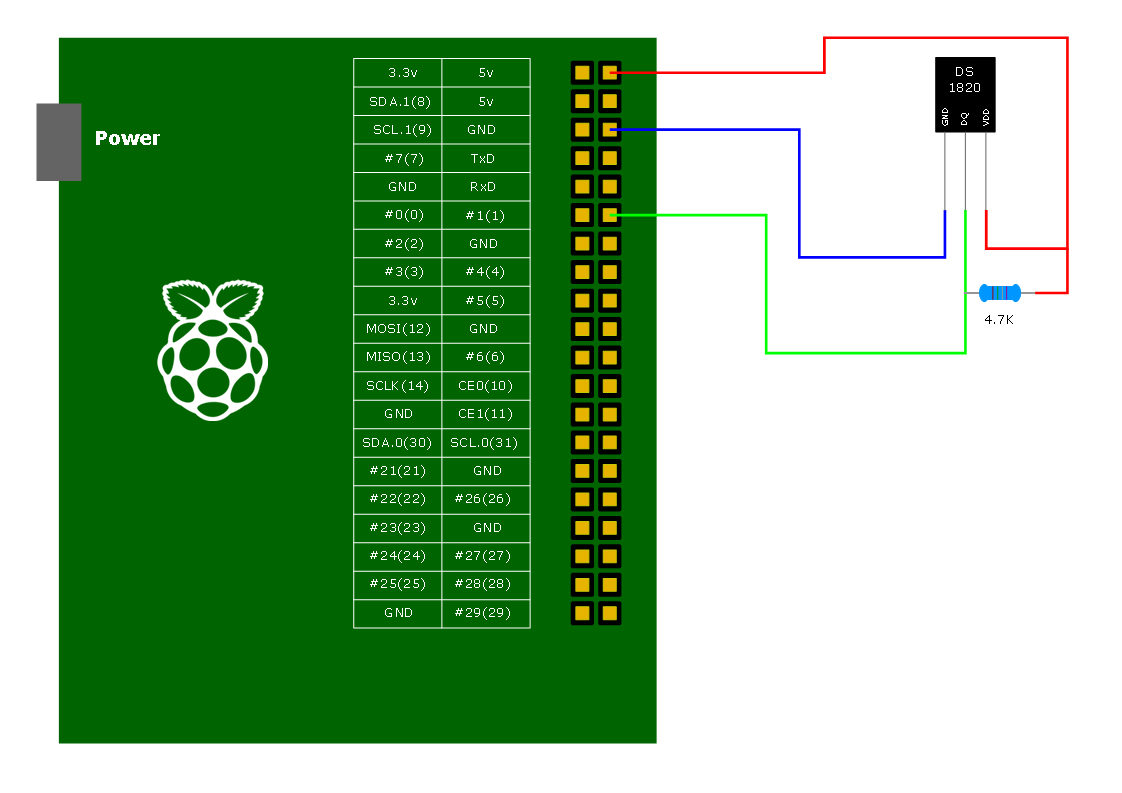
\includegraphics[width=1\textwidth]{./images/raspberry/ds1820_test.png}
\caption{DS1820 Sensor Test}
\label{fig:ds1820_epics_test}
\end{figure}
최종 목표는 다음 Record를 만들어 온습도 값을 읽는 것이다.
\begin{lstlisting}[style=termstyle]
record(ai, "ds1820")       
{
 field(DTYP, "DS1820")
  field(SCAN, "1 second")
  field(INP, "@1")
}
\end{lstlisting}
siteApps안에 ds1820폴더를 만든 후 Base Application을 생성한다.
\begin{lstlisting}[style=termstyle]
pi@raspberrypi cd ../epics/R3.14.12.4/siteApps
pi@raspberrypi ~/epics/R3.14.12.4/siteApps $ mkdir ds1820
pi@raspberrypi ~/epics/R3.14.12.4/siteApps $ cd ds1820
pi@raspberrypi ~/epics/R3.14.12.4/siteApps/ds1820 $ makeBaseApp.pl -t ioc ds1820
pi@raspberrypi ~/epics/R3.14.12.4/siteApps/ds1820 $ makeBaseApp.pl -i -t ioc ds1820

Using target architecture linux-arm (only one available)
The following applications are available:
    ds1820
What application should the IOC(s) boot?
The default uses the IOC's name, even if not listed above.
Application name?

pi@raspberrypi ~/epics/R3.14.12.4/siteApps/ds1820 $ ls
conigure  ds1820App  iocBoot Makefile
\end{lstlisting}
ds1820App/src 폴더로 이동한 후 devDS1820.c 파일을 만들어 기본 코드를 작성한다.
\begin{lstlisting}[style=termstylenumber, caption={Editing \texttt{/etc/fai/NFSROOT}}, label={list:nfsroot-file}]
#include <stdio.h>
#include <string.h>
#include <stdlib.h>

#include <epicsExport.h>
#include <devSup.h>
#include <recSup.h>
#include <recGbl.h>
#include <dbAccess.h>
#include <callback.h>
#include <aiRecord.h>

#include <wiringPi.h>

static long ai_init_record(aiRecord *pai);
static long read_ai(aiRecord *pai);

static long ai_init_record(aiRecord *pai)
{
}

static long read_ai(aiRecord *pai)
{
}

struct
{
  long num;
  DEVSUPFUN     report;
  DEVSUPFUN     init;
  DEVSUPFUN     init_record;
  DEVSUPFUN     get_ioint_info;
  DEVSUPFUN     read_ai;
  DEVSUPFUN     special_linconv;
} devAiDS1820Async = {
  6,
  NULL,
  NULL,
  ai_init_record,
  NULL,
  read_ai,
  NULL
};

epicsExportAddress(dset,devAiDS1820Async);
\end{lstlisting}
기본 구조는 아날로그 입력을 위해 aiRecord를 사용하였으며, 초기화 함수와 센서 값을 읽기 위한 함수로 
구성되어 있다. 또한 wiringPi Library를 사용하기 위해 헤더파일을 추가하였다. dset을 devAiDS1820Async로 
설정하였으므로 devDS1820.dbd 파일을 만들어 다음과 같이 작성한다.
\begin{lstlisting}[style=termstyle]
device(ai, INST_IO, devAiDS1820Async, "DS1820")
\end{lstlisting}
이제 실제 코드를 작성하도록 한다. 우선 코드를 Asynchronous 형식으로 만들기 위해 다음과 같이 Callback 
함수를 만들고 초기화 한다. 
\begin{lstlisting}[style=termstylenumber, caption={Editing \texttt{/etc/fai/NFSROOT}}, label={list:nfsroot-file}]
#include <stdio.h>
#include <string.h>
#include <stdlib.h>

#include <epicsExport.h>
#include <devSup.h>
#include <recSup.h>
#include <recGbl.h>
#include <dbAccess.h>
#include <callback.h>
#include <aiRecord.h>

#include <wiringPi.h>

typedef struct _DS1820_INFO
{
  CALLBACK callback;

}DS1820_INFO;

static long ai_init_record(aiRecord *pai);
static long read_ai(aiRecord *pai);

static void myCallback(CALLBACK *pcallback)
{
  aiRecord *precord;
  struct rset *prset;

  callbackGetUser(precord, pcallback);
  prset = (struct rset *)(precord->rset);

  dbScanLock((dbCommon*)precord);
  (*prset->process)(precord);
  dbScanUnlock((dbCommon*)precord);
}

static long ai_init_record(aiRecord *pai)
{
  DS1820_INFO *ds1820_info = malloc(sizeof(DS1820_INFO));

  callbackSetCallback(myCallback, &ds1820_info->callback);
  callbackSetPriority(priorityLow, &ds1820_info->callback);
  callbackSetUser(pai, &ds1820_info->callback);

  pai->dpvt = ds1820_info;
}

static long read_ai(aiRecord *pai)
{
  DS1820_INFO *ds1820_info = pai->dpvt;

  if(pai->pact)
  {
    pai->udf = FALSE;

    return 2;
  }

  pai->pact = TRUE;
  callbackRequestDelayed(&ds1820_info->callback, pai->disv);

  return 0;

}

struct
{
  long num;
  DEVSUPFUN     report;
  DEVSUPFUN     init;
  DEVSUPFUN     init_record;
  DEVSUPFUN     get_ioint_info;
  DEVSUPFUN     read_ai;
  DEVSUPFUN     special_linconv;
} devAiDS1820Async = {
  6,
  NULL,
  NULL,
  ai_init_record,
  NULL,
  read_ai,
  NULL
};

epicsExportAddress(dset,devAiDS1820Async);
\end{lstlisting}
DS1820\_INFO 구조체는 callback 함수의 포인터를 포함하여 센서에 대한 정보를 저장하기 위한 구조체 이다.
기본적인 준비가 되었으므로 몇가지 초기화 작업을 다음과 같이 추가한다.
\begin{lstlisting}[style=termstylenumber, caption={Editing \texttt{/etc/fai/NFSROOT}}, label={list:nfsroot-file}]
static long ai_init_record(aiRecord *pai)
{
  DS1820_INFO *ds1820_info = malloc(sizeof(DS1820_INFO));

  callbackSetCallback(myCallback, &ds1820_info->callback);
  callbackSetPriority(priorityLow, &ds1820_info->callback);
  callbackSetUser(pai, &ds1820_info->callback);

  if(wiringPiSetup() == -1)
    return 1;

  char *para;
  int pin_num = 0;

  para = pai->inp.value.instio.string;

  pin_num = atoi(para);

  pai->dpvt = ds1820_info;

  return 0;
}
\end{lstlisting}
pin\_num를 read\_ai 함수에서 사용하기 위해 다음과 같이 DS1820\_INFO 구조체에 변수를 추가하고 값을 초기화 
한다.
\begin{lstlisting}[style=termstylenumber, caption={Editing \texttt{/etc/fai/NFSROOT}}, label={list:nfsroot-file}]
struct _DS1820_INFO
{
  CALLBACK callback;

  int pin_num;

}DS1820_INFO;

...
...

static long ai_init_record(aiRecord *pai)
{
  DS1820_INFO *ds1820_info = malloc(sizeof(DS1820_INFO));

  callbackSetCallback(myCallback, &ds1820_info->callback);
  callbackSetPriority(priorityLow, &ds1820_info->callback);
  callbackSetUser(pai, &ds1820_info->callback);

  if(wiringPiSetup() == -1)
    return 1;

  char *para;
  int pin_num = 0;

  para = pai->inp.value.instio.string;

  pin_num = atoi(para);


  ds1820_info->pin_num = pin_num;

  pai->dpvt = ds1820_info;

  return 0;
}
\end{lstlisting}
다음은 read\_ai 함수에 실제 값을 읽어 Record 변수에 저장하는 코드를 추가한다.
\begin{lstlisting}[style=termstylenumber, caption={Editing \texttt{/etc/fai/NFSROOT}}, label={list:nfsroot-file}]
static long read_ai(aiRecord *pai)
{
  DS1820_INFO *ds1820_info = pai->dpvt;

  if(pai->pact)
  {
  readDS1820(ds1820_info);

    pai->val = ds1820_info->temper;

    pai->udf = FALSE;

    return 2;
  }

  pai->pact = TRUE;
  callbackRequestDelayed(&dht_info->callback, pai->disv);

  return 0;
}
\end{lstlisting}
readDS1820 함수는 실제 센서로 부터 온습도 값을 읽은 후 DS1820\_INFO 구조체에 선언된 온습도 변수에 저장하는 
함수로 다음과 같다. 
\begin{lstlisting}[style=termstylenumber, caption={Editing \texttt{/etc/fai/NFSROOT}}, label={list:nfsroot-file}]
void ds1820_read(DS1820_INFO* ds1820_info)
{
  uint8_t busy = 1;
  int pin = ds1820_info->pin_num;

  onewire_reset(pin);
  onewire_write(pin, 0xCC);
  onewire_write(pin, 0x44);

  delay(750);
  while(busy == 0)
  {
    busy = onewire_read(pin);
    printf("busy: %d\n", busy);
  }

  onewire_reset(pin);
  onewire_write(pin, 0xCC);
  onewire_write(pin, 0xBE);

  uint8_t lsb, msb, th, tl, reserved1, reserved2, count_remain, count_per_c, crc;
  float real_temp = 0.0f;
  float pre_real_temp = ds1820_info->temper;
  signed char temp_read = 0;

  lsb = onewire_read(pin);
  msb = onewire_read(pin);
  th = onewire_read(pin);
  tl = onewire_read(pin);
  reserved1 = onewire_read(pin);
  reserved2 = onewire_read(pin);
  count_remain = onewire_read(pin);
  count_per_c = onewire_read(pin);
  crc = onewire_read(pin);

  uint8_t data[] = {lsb, msb, th, tl, reserved1, reserved2, count_remain, count_per_c};

  onewire_reset(pin);

  if(crc_read(data) == crc)
  {
    temp_read = (signed char)(lsb>>1);

    if(msb == 255)
      temp_read = temp_read | 0x80;

    real_temp = (float)temp_read + 0.85f - (float)count_remain/(float)count_per_c;
    real_temp = (int)(real_temp * 10) / 10.0f;

    ds1820_info->temper = real_temp;
    ds1820_info->pre_temper = real_temp;
  }
  else
    ds1820_info->temper = pre_real_temp;

}
\end{lstlisting}
ds1820\_read는 4개의 함수를 내부에서 호출하는데 다음과 같다.
\begin{itemize}
\item onewire\_reset: DS1820 센서를 초기화 한다.
\item onewire\_write: 8bit 정보를 센서로 전송한다.
\item onewire\_read: 8bit 정보를 센서로 부터 읽는다.
\item crc\_read: Cyclical Redundancy Check(CRC) 값을 계산한다.
\end{itemize}
onewire\_reset 함수는 DS1820 센서를 초기화 하는 함수로 다음과 같다.
\begin{lstlisting}[style=termstylenumber, caption={Editing \texttt{/etc/fai/NFSROOT}}, label={list:nfsroot-file}]
int onewire_reset(int pin)
{
  int result;

  pinMode(pin, OUTPUT);

  digitalWrite(pin, LOW);
  delayMicroseconds(480);

  pinMode(pin, INPUT);
  delayMicroseconds(70);

  result = digitalRead(pin);

  delayMicroseconds(410);

  return result;
}
\end{lstlisting}
 onewire\_write 함수는 8bit 정보를 센서로 전송하는 함수로 일정한 Timing에 맞춰 1bit씩 전송 하기위해 
onewire\_write\_bit 함수를 호출한다. 
\begin{lstlisting}[style=termstylenumber, caption={Editing \texttt{/etc/fai/NFSROOT}}, label={list:nfsroot-file}]
void onewire_write(int pin, uint8_t data)
{
  int loop;

  for(loop=0; loop<8; loop++)
  {
    onewire_write_bit(pin, data & 0x01);

    data >>= 1;
  }
}

void onewire_write_bit(int pin, int bit)
{
  pinMode(pin, OUTPUT);

  if(bit)
  {
    digitalWrite(pin, LOW);
    delayMicroseconds(6);
    digitalWrite(pin, HIGH);
    delayMicroseconds(64);
  }
  else
  {
    digitalWrite(pin, LOW);
    delayMicroseconds(60);
    digitalWrite(pin, HIGH);
    delayMicroseconds(10);
  }

}
\end{lstlisting}
 onewire\_read 함수는 onewire\_write 함수와 반대로 onewire\_read\_bit 함수를 통해 1bit씩 총 8bit의 정보를 
센서로 부터 읽어온다. 
\begin{lstlisting}[style=termstylenumber, caption={Editing \texttt{/etc/fai/NFSROOT}}, label={list:nfsroot-file}]
uint8_t onewire_read(int pin)
{
  int loop, result=0;

  for(loop=0; loop<8; loop++)
  {
    result >>= 1;

    if(onewire_read_bit(pin))
      result |= 0x80;
  }

  return result;
}

int onewire_read_bit(int pin)
{
  int result;

  pinMode(pin, OUTPUT);

  digitalWrite(pin, LOW);
  delayMicroseconds(6);

  pinMode(pin, INPUT);
  delayMicroseconds(9);

  result = digitalRead(pin) & 0x01;
  delayMicroseconds(55);

  return result;
}
\end{lstlisting}
read 함수는 데이터의 유효성 Check를 위해 CRC 값을 계산하는 함수로 DS1820 센서는 온도 값 계산을 위해 
64bit의 데이터와 8bit CRC 값을 전송한다. crc\_read 함수는 앞서 전송된 64bit 데이터를 이용하여 CRC 
계산을 하는 함수로 센서로 부터 전송된 마지막 8bit CRC 값과 crc\_read 함수를 통해 계산된 CRC 값이 일치하는 
경우에만 온도 값이 유효하다. 
\begin{lstlisting}[style=termstylenumber, caption={Editing \texttt{/etc/fai/NFSROOT}}, label={list:nfsroot-file}]
uint8_t crc_read(uint8_t *data)
{
 uint8_t i, crc;

 crc = 0x00;

 for(i=0; i<8; i++)
  crc = crc_cal(crc, data[i]);

 return crc;
}

uint8_t crc_cal(uint8_t crc, uint8_t data)
{
  int j;
  for(j=0;j<8;j++) {
      if ((data & 0x01 ) ^ (crc & 0x01)) {
	  // DATA ^ LSB CRC = 1
	  crc = crc>>1;
	  // Set the MSB to 1
	  crc = crc | 0x80;
	  // Check bit 3
	  if (crc & 0x04) {
	      crc = crc & 0xFB; // Bit 3 is set, so clear it
	  } else {
	      crc = crc | 0x04; // Bit 3 is clear, so set it
	  }
	  // Check bit 4
	  if (crc & 0x08) {
	      crc = crc & 0xF7; // Bit 4 is set, so clear it
	  } else {
	      crc = crc | 0x08; // Bit 4 is clear, so set it
	  }
      } else {
	  // DATA ^ LSB CRC = 0
	  crc = crc>>1;
	  // clear MSB
	  crc = crc & 0x7F;
	  // No need to check bits, with DATA ^ LSB CRC = 0, they will remain unchanged
      }
      data = data>>1;
  }

  return crc;
}
\end{lstlisting}
구조체 선언 아래에 전체 함수 이름을 선언해 준다.
\begin{lstlisting}[style=termstylenumber, caption={Editing \texttt{/etc/fai/NFSROOT}}, label={list:nfsroot-file}]
...
...

typedef struct _DS1820_INFO
{
  CALLBACK callback;

  int pin_num;

  float temper;
  float pre_temper;
}DS1820_INFO;

void ds1820_read(DS1820_INFO *ds1820_info);
int onewire_reset(int pin);
void onewire_write(int pin, uint8_t data);
void onewire_write_bit(int pin, int bit);
uint8_t onewire_read(int pin);
int onewire_read_bit(int pin);
uint8_t crc_read();
uint8_t crc_cal(uint8_t crc, uint8_t data);
\end{lstlisting}
전체 코드는 다음과 같다.
\begin{lstlisting}[style=termstylenumber, caption={Editing \texttt{/etc/fai/NFSROOT}}, label={list:nfsroot-file}]
#include <stdio.h>
#include <string.h>
#include <stdlib.h>
#include <stdint.h>

#include <epicsExport.h>
#include <devSup.h>
#include <recSup.h>
#include <recGbl.h>
#include <dbAccess.h>
#include <callback.h>
#include <aiRecord.h>

#include <wiringPi.h>

typedef struct _DS1820_INFO
{
  CALLBACK callback;

  int pin_num;

  float temper;
  float pre_temper;
}DS1820_INFO;

void ds1820_read(DS1820_INFO *ds1820_info);
int onewire_reset(int pin);
void onewire_write(int pin, uint8_t data);
void onewire_write_bit(int pin, int bit);
uint8_t onewire_read(int pin);
int onewire_read_bit(int pin);
uint8_t crc_read();
uint8_t crc_cal(uint8_t crc, uint8_t data);

static long ai_init_record(aiRecord *pai);
static long read_ai(aiRecord *pai);

static void myCallback(CALLBACK *pcallback)
{
  aiRecord *precord;
  struct rset *prset;

  callbackGetUser(precord, pcallback);
  prset = (struct rset *)(precord->rset);

  dbScanLock((dbCommon*)precord);
  (*prset->process)(precord);
  dbScanUnlock((dbCommon*)precord);
}

static long ai_init_record(aiRecord *pai)
{
  DS1820_INFO *ds1820_info = malloc(sizeof(DS1820_INFO));

  callbackSetCallback(myCallback, &ds1820_info->callback);
  callbackSetPriority(priorityLow, &ds1820_info->callback);
  callbackSetUser(pai, &ds1820_info->callback);

  if(wiringPiSetup() == -1)
    return 1;

  char *para;
  int pin_num = 0;

  para = pai->inp.value.instio.string;

  pin_num = atoi(para);

  ds1820_info->temper = 0.0f;
  ds1820_info->pre_temper = 0.0f;

  ds1820_info->pin_num = pin_num;

  pai->dpvt = ds1820_info;

  return 0;
}

static long read_ai(aiRecord *pai)
{
  DS1820_INFO *ds1820_info = pai->dpvt;

  if(pai->pact)
  {
    ds1820_read(ds1820_info);

    pai->val = ds1820_info->temper;

    pai->udf = FALSE;

    return 2;
  }

  pai->pact = TRUE;
  callbackRequestDelayed(&ds1820_info->callback, pai->disv);

  return 0;
}

struct
{
  long num;
  DEVSUPFUN     report;
  DEVSUPFUN     init;
  DEVSUPFUN     init_record;
  DEVSUPFUN     get_ioint_info;
  DEVSUPFUN     read_ai;
  DEVSUPFUN     special_linconv;
} devAiDS1820Async = {
  6,
  NULL,
  NULL,
  ai_init_record,
  NULL,
  read_ai,
  NULL
};

epicsExportAddress(dset,devAiDS1820Async);

void ds1820_read(DS1820_INFO* ds1820_info)
{
  uint8_t busy = 1;
  int pin = ds1820_info->pin_num;

  onewire_reset(pin);
  onewire_write(pin, 0xCC);
  onewire_write(pin, 0x44);

  delay(750);
  while(busy == 0)
  {
    busy = onewire_read(pin);
    printf("busy: %d\n", busy);
  }

  onewire_reset(pin);
  onewire_write(pin, 0xCC);
  onewire_write(pin, 0xBE);

  uint8_t lsb, msb, th, tl, reserved1, reserved2, count_remain, count_per_c, crc;
  float real_temp = 0.0f;
  float pre_real_temp = ds1820_info->temper;
  signed char temp_read = 0;

  lsb = onewire_read(pin);
  msb = onewire_read(pin);
  th = onewire_read(pin);
  tl = onewire_read(pin);
  reserved1 = onewire_read(pin);
  reserved2 = onewire_read(pin);
  count_remain = onewire_read(pin);
  count_per_c = onewire_read(pin);
  crc = onewire_read(pin);

  uint8_t data[] = {lsb, msb, th, tl, reserved1, reserved2, count_remain, count_per_c};

  onewire_reset(pin);

  if(crc_read(data) == crc)
  {
    temp_read = (signed char)(lsb>>1);

    if(msb == 255)
      temp_read = temp_read | 0x80;

    real_temp = (float)temp_read + 0.85f - (float)count_remain/(float)count_per_c;
    real_temp = (int)(real_temp * 10) / 10.0f;

    ds1820_info->temper = real_temp;
    ds1820_info->pre_temper = real_temp;
  }
  else
    ds1820_info->temper = pre_real_temp;

}

int onewire_reset(int pin)
{
  int result;

  pinMode(pin, OUTPUT);

  digitalWrite(pin, LOW);
  delayMicroseconds(480);

  pinMode(pin, INPUT);
  delayMicroseconds(70);

  result = digitalRead(pin);

  delayMicroseconds(410);

  return result;
}

void onewire_write(int pin, uint8_t data)
{
  int loop;

  for(loop=0; loop<8; loop++)
  {
    onewire_write_bit(pin, data & 0x01);

    data >>= 1;
  }
}

void onewire_write_bit(int pin, int bit)
{
  pinMode(pin, OUTPUT);

  if(bit)
  {
    digitalWrite(pin, LOW);
    delayMicroseconds(6);
    digitalWrite(pin, HIGH);
    delayMicroseconds(64);
  }
  else
  {
    digitalWrite(pin, LOW);
    delayMicroseconds(60);
    digitalWrite(pin, HIGH);
    delayMicroseconds(10);
  }

}

uint8_t onewire_read(int pin)
{
  int loop, result=0;

  for(loop=0; loop<8; loop++)
  {
    result >>= 1;

    if(onewire_read_bit(pin))
      result |= 0x80;
  }

  return result;
}

int onewire_read_bit(int pin)
{
  int result;

  pinMode(pin, OUTPUT);

  digitalWrite(pin, LOW);
  delayMicroseconds(6);

  pinMode(pin, INPUT);
  delayMicroseconds(9);

  result = digitalRead(pin) & 0x01;
  delayMicroseconds(55);

  return result;
}

uint8_t crc_read(uint8_t *data)
{
 uint8_t i, crc;

 crc = 0x00;

 for(i=0; i<8; i++)
  crc = crc_cal(crc, data[i]);

 return crc;
}

uint8_t crc_cal(uint8_t crc, uint8_t data)
{
  int j;
  for(j=0;j<8;j++) {
      if ((data & 0x01 ) ^ (crc & 0x01)) {
	  // DATA ^ LSB CRC = 1
	  crc = crc>>1;
	  // Set the MSB to 1
	  crc = crc | 0x80;
	  // Check bit 3
	  if (crc & 0x04) {
	      crc = crc & 0xFB; // Bit 3 is set, so clear it
	  } else {
	      crc = crc | 0x04; // Bit 3 is clear, so set it
	  }
	  // Check bit 4
	  if (crc & 0x08) {
	      crc = crc & 0xF7; // Bit 4 is set, so clear it
	  } else {
	      crc = crc | 0x08; // Bit 4 is clear, so set it
	  }
      } else {
	  // DATA ^ LSB CRC = 0
	  crc = crc>>1;
	  // clear MSB
	  crc = crc & 0x7F;
	  // No need to check bits, with DATA ^ LSB CRC = 0, they will remain unchanged
      }
      data = data>>1;
  }

  return crc;
}
\end{lstlisting}
마지막으로 Makefile에 다음 코드를 추가한 후 make를 실행한다.
\begin{lstlisting}[style=termstyle]
TOP=../..

include $(TOP)/configure/CONFIG
#----------------------------------------
#  ADD MACRO DEFINITIONS AFTER THIS LINE
#=============================

#=============================
# Build the IOC application

USR_INCLUDES += -I/home/pi/wiringPi/wiringPi
wiringPi_DIR += /home/pi/wiringPi/wiringPi /home/pi/wiringPi/devLib

PROD_IOC = ds1820
# dht11.dbd will be created and installed
DBD += ds1820.dbd

# dht11.dbd will be made up from these files:
ds1820_DBD += base.dbd

# Include dbd files from all support applications:
#ds1820_DBD += xxx.dbd
ds1820_DBD += devDS1820.dbd

# Add all the support libraries needed by this IOC
#ds1820_LIBS += xxx

# ds1820_registerRecordDeviceDriver.cpp derives from ds1820.dbd
ds1820_SRCS += ds1820_registerRecordDeviceDriver.cpp
ds1820_SRCS += devDS1820.c

# Build the main IOC entry point on workstation OSs.
ds1820_SRCS_DEFAULT += ds1820Main.cpp
ds1820_SRCS_vxWorks += -nil-

# Add support from base/src/vxWorks if needed
#ds1820_OBJS_vxWorks += $(EPICS_BASE_BIN)/vxComLibrary

# Finally link to the EPICS Base libraries
ds1820_LIBS += $(EPICS_BASE_IOC_LIBS)
ds1820_LIBS += wiringPi

#===========================

include $(TOP)/configure/RULES
#----------------------------------------
#  ADD RULES AFTER THIS LINE
\end{lstlisting}
\begin{lstlisting}[style=termstyle]
pi@raspberrypi ~/epics/R3.14.12.4/siteApps/ds1820/ds1820App/src $ make
\end{lstlisting}
make가 완료되면 bin/linux-arm 폴더에 ds1820 파일이 생성된다.
테스트를 위해 ds1820App/Db 폴더로 이동한 후 처음 테스트 하고자 했던 ds1820.db 파일을 만든다.
\begin{lstlisting}[style=termstyle]
record(ai, "ds1820")
{
  field(DTYP, "DS1820")
  field(SCAN, "1 second")
  field(INP, "@1")
}
\end{lstlisting}
Makefile에 dth11.db를 추가한 후 make를 실행한다.
\begin{lstlisting}[style=termstyle]
TOP=../..
include $(TOP)/configure/CONFIG
#----------------------------------------
#  ADD MACRO DEFINITIONS AFTER THIS LINE

#----------------------------------------------------
#  Optimization of db files using dbst (DEFAULT: NO)
#DB_OPT = YES

#----------------------------------------------------
# Create and install (or just install) into /db
# databases, templates, substitutions like this
#DB += xxx.db
DB += ds1820.db

#----------------------------------------------------
# If .db template is not named *.template add
# _template = 

include $(TOP)/configure/RULES
#----------------------------------------
#  ADD RULES AFTER THIS LINE
\end{lstlisting}
\begin{lstlisting}[style=termstyle]
pi@raspberrypi ~/epics/R3.14.12.4/siteApps/ds1820/ds1820App/Db $ make
\end{lstlisting}
make가 완료되면 최상위 폴더에 db폴더가 만들어지고 그 안에 ds1820.db파일이 생성된다.
\begin{lstlisting}[style=termstyle]
pi@raspberrypi ~/epics/R3.14.12.4/siteApps/ds1820/db $ ls
ds1820.db
\end{lstlisting}
이제 ioc를 실행하기 위해 iocBoot/iocds1820 폴더로 이동한다. st.cmd파일을 수정하기 전 make를 실행해서 
envPahts파일을 만든다.
\begin{lstlisting}[style=termstyle]
pi@raspberrypi ~/epics/R3.14.12.4/siteApps/ds1820/iocBoot/iocds1820 $ make
pi@raspberrypi ~/epics/R3.14.12.4/siteApps/ds1820/iocBoot/iocds1820 $ ls
envPaths  Makefile  st.cmd
\end{lstlisting}
이제 st.cmd파일을 열어 ds1820.db 레코드를 추가해 준다.
\begin{lstlisting}[style=termstyle]
#!../../bin/linux-arm/ds1820

## You may have to change dht11 to something else
## everywhere it appears in this file

< envPaths

cd ${TOP}

## Register all support components
dbLoadDatabase "dbd/ds1820.dbd"
ds1820_registerRecordDeviceDriver pdbbase

## Load record instances
#dbLoadRecords("db/xxx.db","user=piHost")
dbLoadRecords("db/ds1820.db")

cd ${TOP}/iocBoot/${IOC}
iocInit

## Start any sequence programs
#seq sncxxx,"user=piHost"
\end{lstlisting}
최종적으로 st.cmd 파일을 실행파일로 변경한 후 실행한다.
\begin{lstlisting}[style=termstyle]
pi@raspberrypi ~/epics/R3.14.12.4/siteApps/ds1820/iocBoot/iocds1820 $ chmod 755 st.cmd
pi@raspberrypi ~/epics/R3.14.12.4/siteApps/ds1820/iocBoot/iocds1820 $ sudo ./st.cmd
#!../../bin/linux-arm/ds1820
## You may have to change ds1820 to something else
## everywhere it appears in this file
< envPaths
epicsEnvSet("ARCH","linux-arm")
epicsEnvSet("IOC","iocdht11")
epicsEnvSet("TOP","/home/pi/epics/R3.14.12.4/siteApps/ds1820")
epicsEnvSet("EPICS_BASE","/home/pi/epics/R3.14.12.4/base")
cd /home/pi/epics/R3.14.12.4/siteApps/ds1820
## Register all support components
dbLoadDatabase "dbd/ds1820.dbd"
dht11_registerRecordDeviceDriver pdbbase
## Load record instances
#dbLoadRecords("db/xxx.db","user=piHost")
dbLoadRecords("db/ds1820.db")
cd /home/pi/epics/R3.14.12.4/siteApps/ds1820/iocBoot/iocds1820
iocInit
Starting iocInit
############################################################################
## EPICS R3.14.12.4 $Date: Mon 2013-12-16 15:51:45 -0600$
## EPICS Base built Aug 29 2014
############################################################################
iocRun: All initialization complete
## Start any sequence programs
#seq sncxxx,"user=piHost"
epics>
\end{lstlisting}
온도와 습도값이 제대로 읽어지면 끝!
\begin{lstlisting}[style=termstyle]
epics> dbpr ds1820
ASG:                DESC:               DISA: 0             DISP: 0
DISV: 1             NAME: tem           RVAL: 0             SEVR: NO_ALARM
STAT: NO_ALARM      SVAL: 0             TPRO: 0             VAL: 26
\end{lstlisting}

%\clearpage

\bibliographystyle{unsrtnat}

\bibliography{./refs}


\end{document}
